
\chapter[Dạng bài: Xác định thời điểm, số lần qua một vị trí bất kỳ trong dao động điều hòa]{Dạng bài: Xác định thời điểm, số lần qua một vị trí bất kỳ trong dao động điều hòa}
\section{Lý thuyết}
\subsection{Phương pháp sử dụng vòng tròn lượng giác}
\begin{center}
	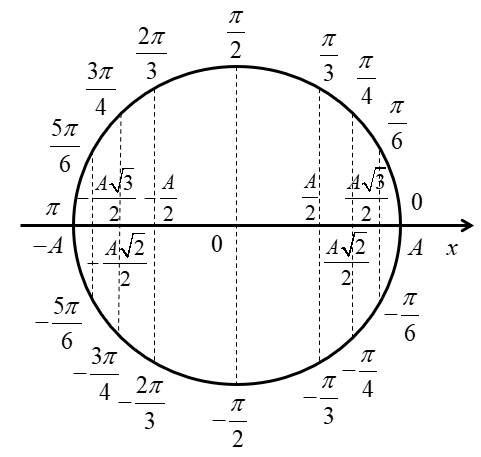
\includegraphics[scale=0.7]{../figs/VN12-PH-02-A-001-1-V2-4.jpg}
\end{center}
\begin{itemize}
	\item Vật dao động điều hòa trên trục O$x$ tương ứng với vật chuyển động tròn đều trên đường tròn tâm O bán kính OA;
	\item Chiều dương của li độ, vận tốc, gia tốc hướng theo chiều của O$x$;
	\item Chiều dương của pha, pha ban đầu ngược chiều kim đồng hồ.
\end{itemize}
\subsection{Một số trường hợp đặc biệt thường gặp}
\begin{center}
	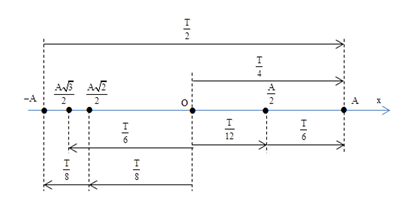
\includegraphics[scale=1]{../figs/VN12-PH-02-A-001-4-V2-2.jpg}
\end{center}
\section{Mục tiêu bài học - Ví dụ minh họa}
\begin{dang}{Sử dụng được phương trình dao động\\ và đường tròn lượng giác để xác định\\ thời điểm vật qua vị trí bất kì}
	\ppgiai{
		\begin{description}
			\item[Bước 1:] Tìm vị trí $x_0$ và chiều chuyển động (dấu của $v_0$) ban đầu của vật tại thời điểm ban đầu $t_0=0$.
			\item[Bước 2:] Sử dụng mối liên hệ giữa dao động điều hòa và chuyển động tròn đều:
			
			Trong một chu kì vật qua vị trí mỗi biên 1 lần, các vị trí khác 2 lần.
			\begin{enumerate}[label=\alph*)]
				\item Nếu vật qua vị trí biên ($x=A$ hoặc $x=-A$)
				\begin{equation*}
					t=(N-1)T+\Delta t_1,
				\end{equation*}
				trong đó:
				\begin{itemize}
					\item $t$ là thời điểm vật đi qua vị trí $x$ đã biết lần thứ $n$ kể từ thời điểm ban đầu $t_0=0$;
					\item $\Delta t_1$ là khoảng thời gian vật đi từ vị trí có li độ $x_0$ đến vị trí biên lần thứ nhất.
					\item $T$ là chu kì của vật.
				\end{itemize}
				\begin{center}
					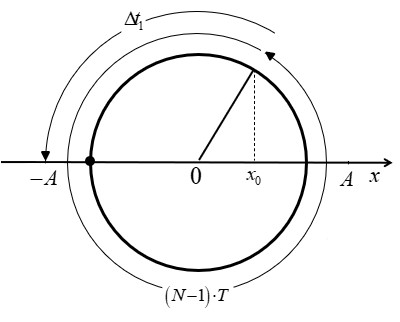
\includegraphics[scale=0.8]{../figs/VN12-PH-02-A-001-4-V2-3.jpg}
				\end{center}
				
				\item Nếu vật qua vị trí khác biên ($x\neq\pm A$) và $n$ lẻ
				\begin{equation*}
					t=\dfrac{N-1}{2}T+\Delta t_1,
				\end{equation*}
				trong đó:
				\begin{itemize}
					\item $t$ là thời điểm vật đi qua vị trí $x$ đã biết lần thứ $n$ kể từ thời điểm ban đầu $t_0=0$;
					\item $\Delta t_1$ là khoảng thời gian vật đi từ vị trí có li độ $x_0$ đến vị trí $x$ lần thứ nhất.
					\item $T$ là chu kì của vật.
				\end{itemize}
				\begin{center}
					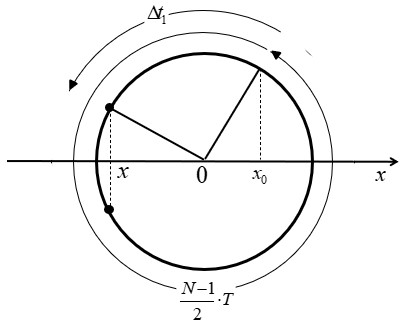
\includegraphics[scale=0.8]{../figs/VN12-PH-02-A-001-4-V2-4.jpg}
				\end{center}
				
				\item Nếu vật qua vị trí khác biên ($x\neq\pm A$) và $n$ chẵn
				\begin{equation*}
					t=\dfrac{N-2}{2}T+\Delta t_2,
				\end{equation*}
				trong đó:
				\begin{itemize}
					\item $t$ là thời điểm vật đi qua vị trí $x$ đã biết lần thứ $n$ kể từ thời điểm ban đầu $t_0=0$;
					\item $\Delta t_2$ là khoảng thời gian vật đi từ vị trí có li độ $x_0$ đến vị trí $x$ lần thứ 2.
					\item $T$ là chu kì của vật.
				\end{itemize}
				\begin{center}
					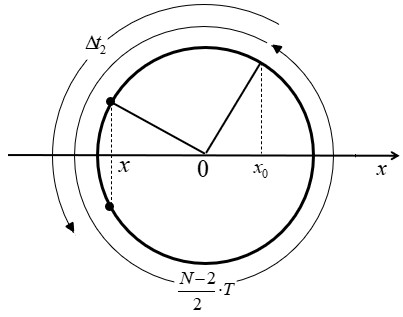
\includegraphics[scale=0.8]{../figs/VN12-PH-02-A-001-4-V2-5.jpg}
				\end{center}
				
			\end{enumerate}
	\end{description}}
	\viduii{3}{Một chất điểm dao động điều hòa theo phương trình $x=4\cos\dfrac{2\pi}{3}t$ ($x$ tính bằng cm; $t$ tính bằng s). Kể từ $t=0$, chất điểm đi qua vị trí có li độ $x=\SI{-2}{\centi\meter}$ lần thứ 2011 tại thời điểm 
		\begin{mcq}(4)
			\item $\SI{3015}{\second}$.
			\item $\SI{6030}{\second}$.
			\item $\SI{3016}{\second}$.
			\item $\SI{6031}{\second}$.
		\end{mcq}
	}
	{\begin{center}
			\textbf{Hướng dẫn giải}
		\end{center}
		
		Chu kì chất điểm dao động điều hòa là
		\begin{equation*}
			T=\dfrac{2\pi}{\omega}=\dfrac{2\pi}{\dfrac{2\pi}{3}\,\text{rad}/\text{s}}=\SI{3}{\second}.
		\end{equation*}
		
		Chất điểm dao động với chu kì $A=\SI{4}{\centi\meter}$ nên vị trí $x=\SI{-2}{\centi\meter}$ không phải là vị trí biên. Do đó, mỗi chu kì, số lần chất điểm dao động điều hòa qua vị trí có li độ $x=\SI{-2}{\centi\meter}$ là 2 lần.
		
		Thời điểm chất điểm dao động điều hòa qua vị trí $x=\SI{-2}{\centi\meter}$ lần thứ 2011 là
		\begin{equation*}
			t=\dfrac{N-1}{2}T+\Delta t_1=1005T+\Delta t_1;
		\end{equation*}
		với $\Delta t_1$ là khoảng thời gian vật đi từ vị trí có li độ $x_0=\SI{4}{\centi\meter}$ đến vị trí $x=\SI{-2}{\centi\meter}$ lần thứ nhất.
		
		\begin{center}
			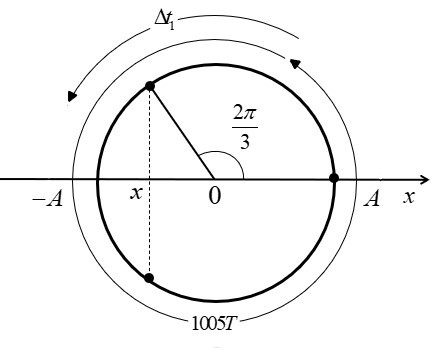
\includegraphics[scale=0.7]{../figs/VN12-PH-02-A-001-4-V2-6.jpg}
		\end{center}
		
		Dựa vào đường tròn lượng giác tai có góc quay từ vị trí vị trí có li độ $x_0=0$ đến vị trí $x=\SI{-2}{\centi\meter}$ lần thứ nhất là $\Delta\alpha=\dfrac{2\pi}{3}\,\text{rad}$, do đó
		\begin{equation*}
			\omega=\dfrac{\Delta\alpha}{\Delta t_1}\Rightarrow\Delta t_1=\dfrac{\Delta\alpha}{	\omega}=\dfrac{\dfrac{2\pi}{3}\,\text{rad}}{\dfrac{2\pi}{3}\,\text{rad}/\text{s}}=\SI{1}{\second}.
		\end{equation*}
		
		Thế $T=\SI{3}{\second}$ và $\Delta t_1=\SI{1}{\second}$ vào biểu thức tính thời điểm chất điểm dao động điều hòa qua vị trí $x=\SI{-2}{\centi\meter}$ lần thứ 2011 ta được
		\begin{equation*}
			t=1005T+\Delta t_1=1005\cdot\SI{3}{\second} +\SI{1}{\second}=\SI{3016}{\second}.
		\end{equation*}
		
		\textbf{Đáp án: C.}
	}
	\viduii{3}{Một vật dao động điều hòa theo phương trình $x=10 \cos(10\pi t) \ \text{cm}$. Thời điểm vật đi qua vị trí N có li độ $x=\SI{5}{cm}$ lần thứ 2009 theo chiều dương là
		\begin{mcq}(4)
			\item $\SI{401,8}{s}$. 		      	
			\item $\SI{408,1}{s}$.			
			\item $\SI{410,8}{s}$.	.	 	
			\item $\SI{401,76}{s}$.
		\end{mcq}
	}
	{\begin{center}
			\textbf{Hướng dẫn giải}
		\end{center}
		
		Chu kỳ dao động:
		\begin{equation*}
			T =\SI{0,2}{s}.
		\end{equation*}
		Ta có ở thời điểm $t=0$ thì
		\begin{equation*}
			x= 10 \cos 0 =\SI{10}{cm}= + A.
		\end{equation*}
		
		Thời gian vật đi từ vị trí ban đầu $x=+A$ tới $x =\SI{5}{cm} =\dfrac{A}{2}$ chuyển động theo chiều dương lần thứ nhất là
		
		\begin{equation*}
			\dfrac{T}{2} + \dfrac{T}{4} + \dfrac{T}{12} = \dfrac{5T}{6}.
		\end{equation*}
		
		Còn 2008 lần sau đó, cứ một chu kì vật lại qua $x=\dfrac{A}{2}$ theo chiều dương một lần nên cần thời gian $2008T$.
		
		Thời điểm vật đi qua vị trí li độ $x=\SI{5}{cm}$ lần thứ 2009 theo chiều dương:
		
		\begin{equation*}
			t =t_1+ 2008T = \SI{401,76}{s}
		\end{equation*}
		
		\textbf{Đáp án: D.}
	}
	
\end{dang}
\begin{dang}{Sử dụng được phương trình dao động và đường tròn lượng giác để xác định số lần vật qua vị trí bất kì}
	\ppgiai{
		\subsubsection{Cách 1}
		\begin{description}
			\item[Bước 1:] Tìm các vị trí $x_1$, $x_2$ và chiều chuyển động (dấu của $v_1$, $v_2$) của vật tại các thời điểm $t_1$, $t_2$.
			\item[Bước 2:] Sử dụng mối liên hệ giữa dao động điều hòa và chuyển động tròn đều: Trong một chu kì vật qua vị trí mỗi biên 1 lần, các vị trí khác 2 lần.
			
			Phân tích:
			\begin{equation*}
				t_2-t_1=nT+\Delta t;
			\end{equation*}
			với $n\in N$ và $0\leq\Delta t<T$.
			
			Gọi $m$ là số lần vật đi qua vị trí  $x$ trong thời gian $\Delta t$ ($m$ có thể nhận 1 trong 3 giá trị: $m=0,1,2$). Để xác định $m$ ta căn cứ vào $x_1$, $x_2$ và dấu của $v_1$, $v_2$.
			
			Kết luận:
			\begin{itemize}
				\item Nếu vật qua vị trí biên ($x=A$ hoặc $x=-A$)
				\begin{equation*}
					N=n+m;
				\end{equation*}
				\item Nếu vật qua vị trí khác biên ($x\neq\pm A$)
				\begin{equation*}
					N=2n+m.
				\end{equation*}
			\end{itemize}
		\end{description}
		
		\subsubsection{Cách 2}	
		\begin{description}
			\item[Bước 1:] Giải phương trình lượng giác
			\begin{equation*}
				x=A\cos(\omega t+\varphi)=t_2-t_1.
			\end{equation*}
			\manatip{
				\begin{equation*}
					\cos x=a\Leftrightarrow \cos x= \cos \alpha\ (-1\leq a \leq 1) \Leftrightarrow \left[
					\begin{matrix}
						x=\alpha+k2\pi\\
						x=-\alpha+k2\pi
					\end{matrix}
					\right.\ (k\in Z)
				\end{equation*}
			}
			\item[Bước 2:] Giải bất phương trình $t_1\leq t\leq t_2$ để tìm ra phạm vi các giá trị của $k$.
			\item[Bước 3:] Tổng số giá trị của $k$ chính là số lần vật đi qua vị trí đó.
		\end{description}	
	}
	\viduii{3}{Một chất điểm dao động điều hòa theo phương trình $x=10\cos\left(5\pi t-\dfrac{\pi}{3}\right)$ ($x$ tính bằng cm, $t$ tính bằng s). Sau khoảng thời gian $\SI{4,2}{\second}$ kể từ $t=0$ chất điểm đi qua vị trí có li độ $x=\SI{-5}{\centi\meter}$ bao nhiêu lần?
		\begin{mcq}(4)
			\item 20 lần.
			\item 10 lần. 
			\item 21 lần.
			\item 11 lần.
		\end{mcq}
		
	}
	{\begin{center}
			\textbf{Hướng dẫn giải}
		\end{center}
		
		\subsubsection{Cách 1:}
		
		Chu kì chất điểm dao động điều hòa là
		\begin{equation*}
			T=\dfrac{2\pi}{\omega}=\dfrac{2\pi}{5\pi\,\text{rad/s}}=\SI{0,4}{\second}.
		\end{equation*}
		
		Phân tích $\SI{4,2}{\second}$ theo chu kì $T$ ta được 
		\begin{equation*}
			\SI{4,2}{\second}=10T+\SI{0,2}{\second}.
		\end{equation*}
		
		Vì chất điểm dao động với chu kì $A=\SI{10}{\centi\meter}$ nên vị trí $x=\SI{-5}{\centi\meter}$ không phải là vị trí biên. Do đó, mỗi chu kì, số lần chất điểm dao động điều hòa qua vị trí có li độ $x=\SI{-5}{\centi\meter}$ là 2 lần.
		
		Số lần chất điểm đi qua vị trí có li độ $x=\SI{-5}{\centi\meter}$ là
		\begin{equation*}
			N=20+m;
		\end{equation*}
		với $m$ là số lần vật đi qua vị trí $x_0=\SI{5}{\centi\meter}$ trong thời gian $\SI{0,2}{\second}$ kể từ $t=0$.
		
		Để xác định $m$ ta căn cứ vào đường tròn lượng giác.
		
		\begin{center}
			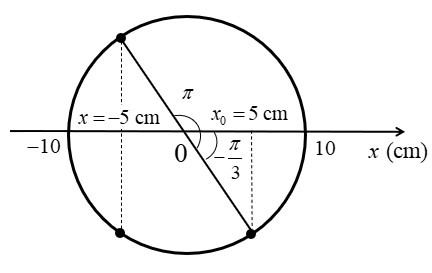
\includegraphics[scale=0.8]{../figs/VN12-PH-02-A-001-4-V2-7.jpg}
		\end{center}
		
		Góc quay vật dao động điều hòa trong khoảng thời gian $\SI{0,2}{\second}$ là
		\begin{equation*}
			\Delta\alpha=\omega t=5\pi\,\text{rad/s}\cdot\SI{0,2}{\second}=\pi\,\text{rad}.
		\end{equation*}
		
		Góc quay vật dao động điều hòa từ vị trí ban đầu $x_0=\SI{5}{\centi\meter}$ đến vị trí $x=\SI{-5}{\centi\meter}$ là $\pi$.
		
		Dựa vào đường tròn lượng giác ta suy ra trong khoảng thời gian $\SI{0,2}{\second}$, kể từ từ vị trí ban đầu $x_0=\SI{-5}{\centi\meter}$ vật đi qua vị trí  $x=\SI{5}{\centi\meter}$ 1 lần. Do đó, $m=1$.
		
		Vậy số lần chất điểm đi qua vị trí có li độ $x=\SI{-5}{\centi\meter}$ kể từ $t=0$ là
		\begin{equation*}
			N=20+1=21.
		\end{equation*}
		\subsubsection{Cách 2:}
		
		Giải phương trình lượng giác
		\begin{eqnarray*}
			&&10\cos\left(5\pi t-\dfrac{\pi}{3}\right)=\SI{-5}{\centi\meter}\\
			&\Leftrightarrow& \cos\left(5\pi t-\dfrac{\pi}{3}\right)=-\dfrac{1}{2}\\
			&\Leftrightarrow& \cos\left(5\pi t-\dfrac{\pi}{3}\right)=\cos \dfrac{2\pi}{3}\\
			&\Leftrightarrow& \left[
			\begin{matrix}
				5\pi t-\dfrac{\pi}{3}&=&\dfrac{2\pi}{3}+k2\pi\\
				5\pi t-\dfrac{\pi}{3}&=&-\dfrac{2\pi}{3}+n2\pi
			\end{matrix}
			\right.\ (k,\ n \in Z)\\
			&\Leftrightarrow& \left[
			\begin{matrix}
				5\pi t-\dfrac{\pi}{3}&=&\dfrac{2\pi}{3}+k2\pi\\
				5\pi t-\dfrac{\pi}{3}&=&-\dfrac{2\pi}{3}+n2\pi
			\end{matrix}
			\right.\ (k,\ n \in Z)\\
			&\Leftrightarrow& \left[
			\begin{matrix}
				t&=&\dfrac{1}{5}+0,4k\\
				t&=&-\dfrac{1}{15}+0,4n
			\end{matrix}
			\right.\ (k,\ n \in Z)
		\end{eqnarray*}
		
		Vì $0\leq t \leq \SI{4,2}{\second}$ nên
		\begin{equation*}
			\left\{
			\begin{matrix}
				k\in\left\lbrace 0;1;2;3;...8;9;10\right\rbrace\\
				n\in\left\lbrace 1;2;3;...8;9;10 \right\rbrace.
			\end{matrix}
			\right.
		\end{equation*}
		
		Vậy có 11 giá trị $k$ và 10 giá trị $n$. Do đó, số lần chất điểm đi qua vị trí có li độ $x=\SI{-5}{\centi\meter}$ kể từ $t=0$ là
		\begin{equation*}
			N=11+10=21.
		\end{equation*}
		
		\textbf{Đáp án: C.}
	}
	
	\viduii{3}{Một chất điểm dao động điều hòa theo phương trình $x=3 \sin\left(5\pi t +\dfrac{\pi}{6}\right)\ \text{cm}$ ($x$ tính bằng cm và $t$ tính bằng giây). Trong một giây đầu tiên từ thời điểm $t=\SI{0,2}{s}$, chất điểm đi qua vị trí có li độ $x=+ \SI{1}{cm}$ là
		\begin{mcq}(4)
			\item 7 lần. 	       		
			\item 6 lần. 		
			\item 4 lần. 			
			\item 5 lần.
		\end{mcq}
		
	}
	{\begin{center}
			\textbf{Hướng dẫn giải}
		\end{center}
		
		Ta có
		\begin{equation*}
			x=3\sin \left (5\pi t +\dfrac{\pi}{6}\right) = 3 \cos \left (5\pi t + \dfrac{\pi}{6}- \dfrac{\pi}{2}\right) = 3\cos \left (5\pi t - \dfrac{\pi}{3}\right)\ \text{cm}.
		\end{equation*}
		Chu kỳ dao động: 
		\begin{equation*} 
			T =\dfrac{2\pi}{\omega} =\SI{0,4}{s}.
		\end{equation*}
		Tại $t =\SI{0,2}{s}$:
		
		\begin{equation*}
			x=3\cos \left(5\pi \text{0,2} -\dfrac{\pi}{3}\right).
		\end{equation*}
		
		\begin{equation*}
			v= - A\omega \sin \left(5\pi \text{0,2}-\dfrac{\pi}{3}\right).
		\end{equation*}
		Suy ra:
		\begin{equation*}
			x= -\SI{1,5}{cm}; v<0.
		\end{equation*}
		Ta có: 
		\begin{equation*}
			\SI{1}{s} = 2T+\dfrac{T}{2}.
		\end{equation*}
		Trong một chu kỳ, vật đi qua vị trí $+\SI{1}{cm}$ 2 lần.
		\begin{center}
			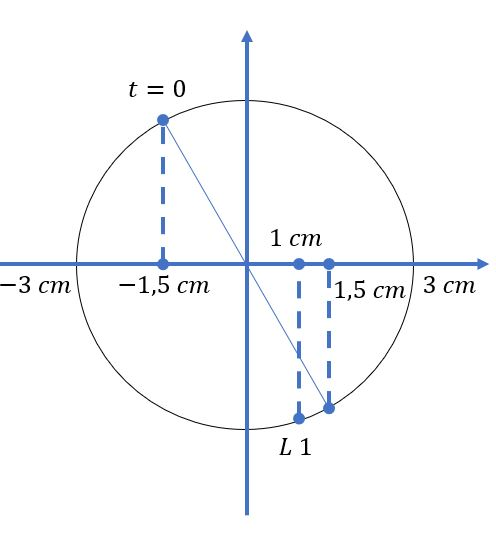
\includegraphics[scale=0.6]{../figs/VN12-PH-02-A-001-4-V2-8.jpg}
		\end{center}
		Trong khoảng thời gian $\dfrac{T}{2}$ vật qua vị trí $+ \SI{1}{cm}$ 1 lần kể từ $t=\SI{0,2}{s}$.
		
		Vậy trong $\SI{1}{s}$ đầu tiên kể từ $t =\SI{0,2}{s}$, vật qua vị trí $+ \SI{1}{cm}$ số lần là $2 \cdot 2 + 1 = 5$ lần.
		
		\textbf{Đáp án: D.}
	}
\end{dang}